\documentclass[a4paper,11pt]{article}
\usepackage{amsmath}

\usepackage{xcolor}
\usepackage{soul}
\usepackage{graphicx}
\usepackage{geometry}
\usepackage{float}

\usepackage[labelfont=bf,skip=0pt]{subcaption}
\usepackage[labelfont=bf,skip=0pt]{caption}
\DeclareCaptionFormat{myformat}{\fontsize{8}{8}\selectfont#1#2#3}
\captionsetup{format=myformat}

\newcommand{\hlc}[2][yellow]{{%
    \colorlet{foo}{#1}%
    \sethlcolor{foo}\hl{#2}}%
}

\usepackage{titling}
\setlength{\droptitle}{-2cm}
\title{CombiFF}
\author{Marina P. Oliveira, Salom\'e Rieder, Philippe H. Hünenberger}
\date{}

\geometry{verbose,a4paper,tmargin=20mm,bmargin=20mm,lmargin=15mm,rmargin=15mm}

\begin{document}
\pagestyle{plain}
\maketitle

%================================================================================
\section{\texttt{CombiFF} Workflow}
%================================================================================

The \texttt{CombiFF} workflow is illustrated in \reffig{cff_workflow}
%
\begin{figure}[h!]
\begin{center}
  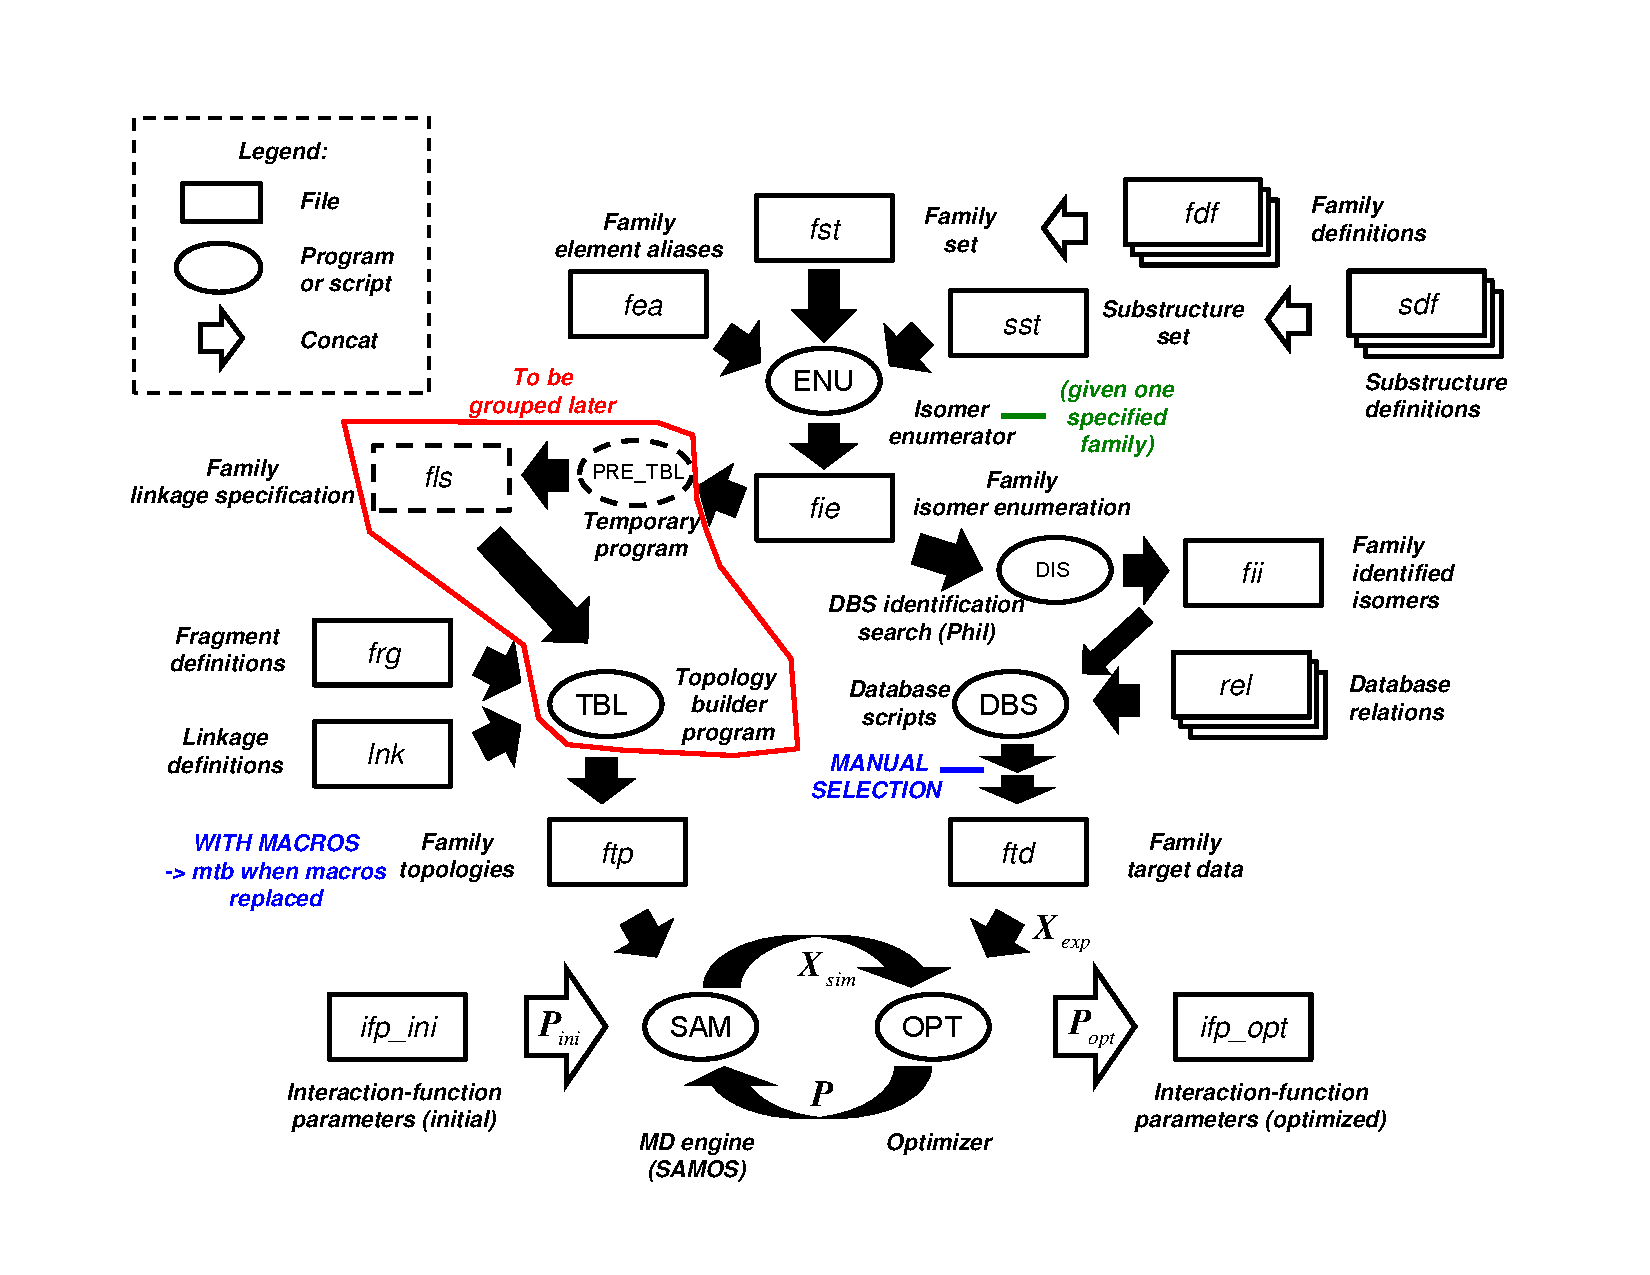
\includegraphics[clip=true,scale=0.6]{fig/cff_workflow.pdf}
\end{center}
\caption{XXX}
\label{cff_workflow}
\end{figure}
%

%================================================================================
\newsec{\texttt{CombiFF} Programs}
%================================================================================

The programs/scripts involved in \texttt{CombiFF} 
summarized in \reftab{programs} and described 
in the following subsections.

\begin{table}[h!]
\begin{center}
\scalebox{0.8}{
\begin{tabular}{|l|l|}
\hline\hline
\multicolumn{2}{|c|}{Programs/scripts involved in \texttt{CombiFF}}\\
\hline
\texttt{ENU} &  isomer enumerator \\
\texttt{PRE\_TBL} &  (temporary) convers \texttt{fie} (SMILES) to fls (ancient \texttt{mol} file, input of \texttt{TBL}) \\
\texttt{TBL} &  topology builder \\
\texttt{DIS} &  (Phil-to-write) scans DBS to map \texttt{fie} (SMILES) to idendtifiers (name, CAS, InChi, InChiKey, ...) \\
\texttt{DBS} &  scripts of the experimental database \\
\texttt{SAM} &  MD engine (SAMOS) \\
\texttt{OPT} &  parameter optimizer \\
\salome{\texttt{CNV}} & \salome{converter and canonicalization program} \\
\hline\hline
\end{tabular}
}
\end{center}
\caption{XXX}
\labtab{programs}
\end{table}



\end{document}



